\documentclass[12pt, twoside]{article}
\documentclass[12pt, twoside]{article}
\usepackage[letterpaper, margin=1in, headsep=0.2in]{geometry}
\setlength{\headheight}{0.6in}
%\usepackage[english]{babel}
\usepackage[utf8]{inputenc}
\usepackage{microtype}
\usepackage{amsmath}
\usepackage{amssymb}
%\usepackage{amsfonts}
\usepackage{siunitx} %units in math. eg 20\milli\meter
\usepackage{yhmath} % for arcs, overparenth command
\usepackage{tikz} %graphics
\usetikzlibrary{quotes, angles}
\usepackage{graphicx} %consider setting \graphicspath{{images/}}
\usepackage{parskip} %no paragraph indent
\usepackage{enumitem}
\usepackage{multicol}
\usepackage{venndiagram}

\usepackage{fancyhdr}
\pagestyle{fancy}
\fancyhf{}
\renewcommand{\headrulewidth}{0pt} % disable the underline of the header
\raggedbottom
\hfuzz=2mm %suppresses overfull box warnings

\usepackage{hyperref}

\fancyhead[LE]{\thepage}
\fancyhead[RO]{\thepage \\ Name: \hspace{4cm} \,\\}
\fancyhead[LO]{BECA / Dr. Huson / Geometry\\*  Unit 10: Trigonometry \\* 2 May 2023}

\begin{document}

\subsubsection*{10.7 Quiz: The tangent function \hfill CCSS.HSG.SRT.C.8}
You must write an equation before solving it. Figures are not necessarily drawn to scale.
\begin{enumerate}
\item Given right $\triangle ABC$ with $AC=10$, m$\angle A=40^\circ$. Find the value of $BC=x$.
  \begin{flushright}
  \begin{tikzpicture}[scale=0.8]
    \draw[thick] (0,0)node[below]{$A$}--
      (6,0)node[below]{$C$}--
      (6,5)node[above]{$B$}--cycle;
    \draw (6,0)++(-0.6,0)--++(0,0.6)--+(0.6,0);
    \node at (3,0)[below]{$10$};
    \node at (6,2.5)[right]{$x$};
    \draw (1,0) arc (0:40:1)node[pos=0.7,right]{$40^\circ$};
  \end{tikzpicture}
  \end{flushright}

\item The right $\triangle ABC$ has a height of $BC=17$ and m$\angle A=58^\circ$. Find the length of its base $AC=x$.
  \begin{flushright}
  \begin{tikzpicture}[scale=0.7]
    \draw[thick] (0,0)node[below]{$A$}--
      (5,0)node[below]{$C$}--
      (5,8)node[above]{$B$}--cycle;
    \draw (5,0)++(-0.6,0)--++(0,0.6)--+(0.6,0);
    \node at (2.5,0)[below]{$x$};
    \node at (5,4)[right]{$17$};
    \draw (1,0) arc (0:58:1)node[pos=0.7,right]{$58^\circ$};
  \end{tikzpicture}
  \end{flushright}

\item The lengths of the legs of right $\triangle ABC$ are $AC=50$ and $BC=25$. Find m$\angle A=x$.
  \begin{flushright}
  \begin{tikzpicture}[scale=1]
    \draw[thick] (0,0)node[below]{$A$}--
      (6,0)node[below]{$C$}--
      (6,3)node[above]{$B$}--cycle;
    \draw (6,0)++(-0.5,0)--++(0,0.5)--+(0.5,0);
    \node at (3,0)[below]{$50$};
    \node at (6,1.5)[right]{$25$};
    \draw (1,0) arc (0:27:1)node[pos=0.7,right]{$x^\circ$};
  \end{tikzpicture}
  \end{flushright}

\newpage
\item The dimensions of right $\triangle ABC$ are $AC=12$ and $BC=5$. Find length of the hypotenuse $AB=x$.
  \begin{flushright}
  \begin{tikzpicture}[scale=1]
    \draw[thick] (0,0)node[below]{$A$}--
      (6,0)node[below]{$C$}--
      (6,3)node[above]{$B$}--cycle;
    \draw (6,0)++(-0.4,0)--++(0,0.4)--+(0.4,0);
    \node at (3,0)[below]{$12$};
    \node at (6,1.5)[right]{$5$};
    \node at (3.1,2)[right]{$x$};
  \end{tikzpicture}
  \end{flushright}

\item The hypotenuse of right $\triangle ABC$ is 20.0 units long and the triangle's height is 17.3 units. Find the length of its base $AC=x$, to the \emph{nearest tenth}.
  \begin{flushright}
  \begin{tikzpicture}[scale=0.7]
    \draw[thick] (0,0)node[below]{$A$}--
      (5,0)node[below]{$C$}--
      (5,8)node[above]{$B$}--cycle;
    \draw (5,0)++(-0.6,0)--++(0,0.6)--+(0.6,0);
    \node at (2.5,0)[below]{$x$};
    \node at (5,4)[right]{$17.3$};
    \node at (1.6,4.3)[below, rotate=58]{$20.0$};
  \end{tikzpicture}
  \end{flushright}

\subsubsection*{Find $x$ to the \emph{nearest tenth}.}
  \begin{multicols}{2}
  \item $\displaystyle \tan 80^\circ = \frac{x}{12}$ \vspace{3cm}
  \item $\displaystyle \tan 30^\circ = \frac{10}{x}$ \vspace{4cm}
  \end{multicols} \vspace{2cm}
\subsubsection*{Find $\theta$ to the \emph{nearest whole degree}.}
  \begin{multicols}{2}
  \item $\displaystyle \theta = \tan^{-1} (\frac{7}{9})$ \vspace{3cm}
  \item $\displaystyle \tan \theta = \frac{1}{1.73}$ \vspace{3cm}
  \end{multicols}

\newpage
\subsubsection*{Modeling situations with right triangles \hfill HSG.MG.A.1}
\item A tree casts a shadow 12 feet long. The angle of elevation from the tip of the shadow to the top of the tree is $70^\circ$. To the nearest foot, how tall is the tree?
  \begin{flushright}
  \begin{tikzpicture}[scale=1]
    \draw[thick] (0,0)--
      (3,0)--
      (3,7)--cycle;
    \draw (3,0)++(-0.4,0)--++(0,0.4)--+(0.4,0);
    \node at (1.5,0)[below]{$12$ feet};
    \node at (3,3)[right]{$x$};
    \draw (0.5,0) arc (0:65:0.5)node[pos=0.7,right]{$70^\circ$};
  \end{tikzpicture}
  \end{flushright}

\item From the top of a hill a dog is visible at an angle of depression of $34^\circ$. If the hill is 11 meters tall, determine the distance from the dog to the base of the hill, \emph{x}, to the \emph{nearest meter}.
\begin{center}
    \begin{tikzpicture}[scale=1.1]
      \draw [thick] (10,0)--(0,0)--(10,2.0)--cycle;
      \draw (10,0)++(-0.3,0)--++(0,0.3)--+(0.3,0);
      \draw [dashed, <-] (5,2)--(10,2.0);
      \draw [thick, ->] (8.5,2) arc [start angle=180, end angle=191.3, radius=1.5];
      \node at (5.5,2)[below]{Angle of depression $=34^\circ$};
      \node at (10,1)[left]{$h=11$};
      \node at (6,0)[below]{$x$};
      \node at (0,0)[below]{Dog};
    \end{tikzpicture}
  \end{center}

\newpage
\item A drone flying at an altitude of 1,800 meters is observed twice. The first time the angle of elevation is $7.2^\circ$ and exactly one minute later the angle of elevation is $9.7^\circ$. \\[0.25cm]
Find the distance the drone flies over the minute and its speed in kilometers per hour.

\hfill (\emph{not drawn to scale})
\begin{center}
  \begin{tikzpicture}[scale=1.1]
    \draw [thick] (10,0)--(0,0)--(10,2.0)--cycle;
    \draw (10,0)++(-0.3,0)--++(0,0.3)--+(0.3,0);
    \draw [dashed] (0,0)--(7,2.0);
    \draw [dashed, <-] (6,2)--(10,2);
    \draw [thick, ->] (1.5,0) arc [start angle=0, end angle=11.3, radius=1.5];
    \draw [thick, ->] (2.5,0) arc [start angle=0, end angle=15.3, radius=2.5];
    \node at (1,0.7)[above]{Angles of elevation};
    \node at (1.5,0)[below]{$7.2^\circ$};
    \node at (3,0)[above]{$9.7^\circ$};
    \node at (10,1.2)[left]{$1800$};
    \node at (8,2)[above]{drone};
  \end{tikzpicture} 
\end{center}
\vspace{11cm}

\subsubsection*{Spicy: Radian measures \hfill HSN.A.Q.1 Use units in formulas}
\begin{multicols}{2}
  \item Convert $30^\circ$ to radians, to the \\
  \emph{nearest thousandth}. \vspace{2cm}
  \item Convert $\frac{1}{4}\pi$ radians to degrees. \vspace{2cm}
\end{multicols}

\end{enumerate}
\end{document}
